\documentclass[11pt,a4paper]{article}
\usepackage[T1]{fontenc}
\usepackage[utf8]{inputenc}
\usepackage[spanish,es-tabla]{babel}
\usepackage[margin=2.4cm]{geometry}
\usepackage{graphicx}
\usepackage{amsmath}
\usepackage{booktabs}
\usepackage{xcolor}
\usepackage{listings}
\usepackage[hidelinks]{hyperref}
\graphicspath{{../images/}{../resultados/}}
\setlength{\parindent}{0pt}
\setlength{\parskip}{4pt}
\setlength{\emergencystretch}{2em}
\lstset{language=Python,basicstyle=\ttfamily\footnotesize,
  keywordstyle=\color{blue!50!black},commentstyle=\color{black!55},
  stringstyle=\color{green!35!black},showstringspaces=false,
  breaklines=true,columns=fullflexible,keepspaces=true,
  frame=single,rulecolor=\color{black!20},tabsize=4}
\title{Lectura de im\'agenes y conversi\'on a escala de grises con OpenCV}
\author{Camilo Eduardo Mu\~noz Albornoz\\
    Procesamiento Digital de Im\'agenes}
\date{}

\begin{document}
\maketitle

\begin{abstract}
Se estudia la representaci\'on de una imagen en los formatos PNG, JPG, BMP
y TIFF, y su conversi\'on a escala de grises mediante dos ecuaciones
implementadas con ciclos y la funci\'on nativa de OpenCV. Se comparan el
tama\~no en disco, la memoria de las matrices, la apariencia visual y la
intensidad promedio. Los resultados muestran diferencias importantes de
almacenamiento entre formatos y una gran similitud entre la ponderaci\'on
NTSC y OpenCV. Para el paisaje analizado, el promedio de los canales
produce una imagen de menor intensidad media.
\end{abstract}

\section*{Introducci\'on}
Una imagen digital puede almacenarse con distintas codificaciones sin que
su representaci\'on decodificada tenga necesariamente dimensiones diferentes.
Por otra parte, convertir una imagen a escala de grises exige definir
c\'omo se combina la informaci\'on de sus canales. Este taller relaciona
ambos aspectos mediante un paisaje con cielo, monta\~nas, vegetaci\'on y lago.
El trabajo se desarroll\'o en Python con OpenCV.

\section{Objetivo}
Analizar la lectura, representaci\'on, conversi\'on y almacenamiento de
im\'agenes digitales con OpenCV, comparando distintos formatos y tres
m\'etodos de conversi\'on a escala de grises.
\begin{itemize}
  \item Cargar el mismo paisaje en PNG, JPG, BMP y TIFF, y comparar sus
  propiedades en memoria y en disco.
  \item Implementar mediante ciclos las ecuaciones NTSC y de promedio
  propuestas, respetando el orden BGR de OpenCV.
  \item Obtener y guardar una conversi\'on nativa con
  \texttt{cv.COLOR\_BGR2GRAY}.
  \item Interpretar las diferencias visuales y cuantificarlas mediante
  la intensidad promedio.
\end{itemize}

\section{Algoritmos utilizados}
\subsection{Lectura y caracterizaci\'on de formatos (punto 1)}
Se carg\'o cada archivo con \texttt{cv.imread}. Antes de consultar sus
propiedades se verific\'o que la lectura fuera v\'alida. El atributo
\texttt{nbytes} mide los bytes de los elementos de la matriz, mientras que
\texttt{os.path.getsize} mide el archivo almacenado.
\begin{lstlisting}
import cv2 as cv
import os

archivos = [
    "images/paisaje.png",
    "images/paisaje.jpg",
    "images/paisaje.bmp",
    "images/paisaje.tiff"
]

for archivo in archivos:
    image = cv.imread(archivo)
    if image is None:
        print("No se pudo cargar:", archivo)
        continue

    print("Archivo:", archivo)
    print("Dimensiones:", image.shape)
    print("Tipo de datos:", image.dtype)
    print("Numero de elementos:", image.size)
    print("Memoria de la matriz:", image.nbytes, "bytes")
    print("Tamano del archivo:", os.path.getsize(archivo), "bytes")
\end{lstlisting}

\subsection{Conversiones manuales con ciclos (punto 3)}
Se aplicaron las ecuaciones solicitadas, denominadas en el taller NTSC
y promedio RGB, respectivamente:
\begin{align}
Y_{\mathrm{NTSC}} &= 0.2989R + 0.5870G + 0.1140B,\label{eq:ntsc}\\
Y_{\mathrm{prom}} &= 0.333R + 0.333G + 0.333B.\label{eq:prom}
\end{align}
Los siguientes fragmentos corresponden a las dos funciones del notebook.
Cada una recorre la imagen por filas y columnas, separa los canales BGR
que OpenCV entrega al leer una imagen y asigna la intensidad calculada a
los tres canales de salida.
\begin{lstlisting}
def convertir_a_gris_NTSC(image):
    if image is None:
        raise ValueError("La imagen proporcionada es None.")

    image_gris = image.copy()
    alto, ancho = image_gris.shape[:2]

    for y in range(alto):
        for x in range(ancho):
            pixel = image_gris[y, x]
            B = pixel[0]
            G = pixel[1]
            R = pixel[2]
            Y = int(0.2989 * R + 0.5870 * G + 0.1140 * B)
            image_gris[y, x] = [Y, Y, Y]

    return image_gris

def convertir_a_gris_promedio(image):
    if image is None:
        raise ValueError("La imagen proporcionada es None.")

    image_gris = image.copy()
    alto, ancho = image_gris.shape[:2]

    for y in range(alto):
        for x in range(ancho):
            pixel = image_gris[y, x]
            B = pixel[0]
            G = pixel[1]
            R = pixel[2]
            Y = int(0.333 * R + 0.333 * G + 0.333 * B)
            image_gris[y, x] = [Y, Y, Y]

    return image_gris

image = cv.imread("images/paisaje.png")
image_gris_NTSC = convertir_a_gris_NTSC(image)
image_gris_promedio = convertir_a_gris_promedio(image)
\end{lstlisting}

\subsection{Conversi\'on nativa y almacenamiento (puntos 4 y 5)}
Se utiliz\'o \texttt{cv.cvtColor} para obtener la conversi\'on nativa y se
guardaron las tres im\'agenes resultantes en formato PNG.
\begin{lstlisting}
def convertir_a_gris(image):
    if image is None:
        raise ValueError("La imagen proporcionada es None.")

    image_gris = image.copy()
    image_gris = cv.cvtColor(image_gris, cv.COLOR_BGR2GRAY)
    return image_gris

image = cv.imread("images/paisaje.png")
image_gris = convertir_a_gris(image)
os.makedirs("resultados", exist_ok=True)

cv.imwrite("resultados/paisaje_gris_ntsc.png", image_gris_NTSC)
cv.imwrite("resultados/paisaje_gris_promedio.png", image_gris_promedio)
cv.imwrite("resultados/paisaje_gris.png", image_gris)
\end{lstlisting}
Los archivos guardados corresponden a las im\'agenes generadas en los
ejercicios anteriores.

\subsection{Medici\'on de intensidad (punto 6)}
Para una imagen de alto $H$ y ancho $W$, la intensidad promedio es
\begin{equation}
\overline{Y}=\frac{1}{HW}\sum_{y=0}^{H-1}\sum_{x=0}^{W-1}Y(y,x).
\end{equation}
En esta expresi\'on, $Y(y,x)$ representa el valor de intensidad del p\'ixel
ubicado en la fila $y$ y la columna $x$. En una imagen en escala de grises,
cada p\'ixel tiene un solo valor entre 0 y 255: el valor 0 corresponde al
negro y el valor 255 al blanco. Las sumatorias agregan todos los valores de
los $H\times W$ p\'ixeles y la divisi\'on por $HW$ calcula su media
aritm\'etica. Por eso, $\overline{Y}$ resume el brillo promedio de toda la
imagen: valores mayores indican una imagen globalmente m\'as clara y valores
menores una imagen globalmente m\'as oscura.

En el programa, las im\'agenes en escala de grises se almacenan como matrices
de NumPy. El m\'etodo \texttt{mean()} suma internamente todos los elementos de
la matriz y los divide por la cantidad total de elementos. Por lo tanto,
\texttt{image\_gris.mean()} implementa directamente la ecuaci\'on anterior,
porque la matriz contiene un valor $Y(y,x)$ por cada p\'ixel. En las salidas
manuales los tres canales contienen el mismo valor $Y$, de modo que su media
es equivalente a calcular la media de un solo canal.
\begin{lstlisting}
print("----- BRILLO PROMEDIO -----")
print("NTSC:", image_gris_NTSC.mean())
print("Promedio RGB:", image_gris_promedio.mean())
print("OpenCV:", image_gris.mean())

ntsc_1_canal = image_gris_NTSC[:, :, 0]
diferencia = cv.absdiff(ntsc_1_canal, image_gris)
print("Diferencia promedio NTSC vs OpenCV:", diferencia.mean())
print("Diferencia maxima NTSC vs OpenCV:", diferencia.max())
\end{lstlisting}
Las salidas manuales tienen tres canales id\'enticos, de modo que su
media sobre todos los elementos coincide con la media de un solo canal.
Para comparar p\'ixel a p\'ixel con OpenCV se selecciona uno de ellos.
\texttt{cv.absdiff} evita el desbordamiento que puede ocurrir al restar
directamente matrices \texttt{uint8}.

\section{Consideraciones y explicaci\'on de la t\'ecnica}
\subsection{Representaci\'on y compresi\'on}
La imagen original mide $800\times533$ p\'ixeles. OpenCV la carga como
una matriz \texttt{uint8} de forma $(533,800,3)$, en orden alto, ancho y
canales. La lectura a color utilizada entrega los canales en orden BGR:
el \mbox{\texttt{pixel[0]}} es azul, \texttt{pixel[1]} es verde y
\texttt{pixel[2]} es rojo. Sus elementos ocupan
\[
533\times800\times3\times1\ \text{byte}=1\,279\,200\ \text{bytes}.
\]
Esta cifra corresponde al contenido de la matriz; no representa toda la
memoria utilizada por Python o por el proceso de decodificaci\'on.

PNG utiliza compresi\'on sin p\'erdida y JPG emplea compresi\'on con
p\'erdida. BMP suele almacenar datos sin comprimir y TIFF admite diversas
codificaciones y opciones de compresi\'on. El tama\~no de un TIFF, por
s\'i solo, no permite identificar su compresi\'on ni demostrar fidelidad
respecto a una fuente. Adem\'as, guardar en un formato sin p\'erdida no
recupera informaci\'on perdida previamente.

\subsection{Ponderaci\'on, cuantizaci\'on y canales}
La conversi\'on documentada por OpenCV usa
$Y=0.299R+0.587G+0.114B$~\cite{opencv}. Su cercan\'ia con
la ecuaci\'on~\eqref{eq:ntsc} explica la similitud visual. No obstante,
el coeficiente rojo es ligeramente diferente y el c\'odigo manual aplica
\texttt{int()}, que trunca los valores no negativos. La cuantizaci\'on
de la salida nativa tambi\'en influye en las diferencias observadas.

Los pesos NTSC del taller suman $0.9999$ y los del promedio suman
$0.999$. Por tanto, la ecuaci\'on~\eqref{eq:prom} es una aproximaci\'on
al promedio aritm\'etico $(R+G+B)/3$. Se mantuvieron los coeficientes
solicitados; esta aproximaci\'on y el truncamiento introducen un peque\~no
sesgo hacia intensidades menores.

En los m\'etodos manuales, los valores $[Y,Y,Y]$ producen una apariencia
gris, pero conservan la forma $(533,800,3)$ y los $1\,279\,200$ bytes de
datos. La conversi\'on nativa produce una matriz de un canal con forma
$(533,800)$ y $426\,400$ bytes. Ambos casos representan intensidades
enteras en el rango de 0 (negro) a 255 (blanco). La media se usa aqu\'i
como indicador de intensidad digital, no como medici\'on f\'isica de
luminancia ni como medida completa de brillo percibido.

\section{Im\'agenes generadas y resultados}
\subsection{Formatos y comparaci\'on visual (puntos 1 y 2)}
La Tabla~\ref{tab:formatos} recoge los resultados registrados en el
notebook. Todos los archivos cargados tienen forma $(533,800,3)$,
tipo \texttt{uint8} y $1\,279\,200$ elementos.
\begin{table}[htbp]
\centering
\caption{Tama\~no de los archivos y de las matrices decodificadas.}
\label{tab:formatos}
\begin{tabular}{lrr}
\toprule
Formato & Archivo (bytes) & Datos en RAM (bytes)\\
\midrule
PNG  & $876\,700$   & $1\,279\,200$\\
JPG  & $192\,680$   & $1\,279\,200$\\
BMP  & $1\,279\,338$ & $1\,279\,200$\\
TIFF & $1\,279\,480$ & $1\,279\,200$\\
\bottomrule
\end{tabular}
\end{table}

En la observaci\'on realizada durante el taller, las cuatro versiones
se percibieron visualmente muy similares. Esta apreciaci\'on no demuestra
igualdad de p\'ixeles: en particular, JPG puede introducir cambios por
la compresi\'on con p\'erdida. Tener las mismas dimensiones y tipo de
dato tampoco implica contener los mismos valores.

\begin{figure}[htbp]
\centering
\begin{minipage}{0.48\textwidth}
\centering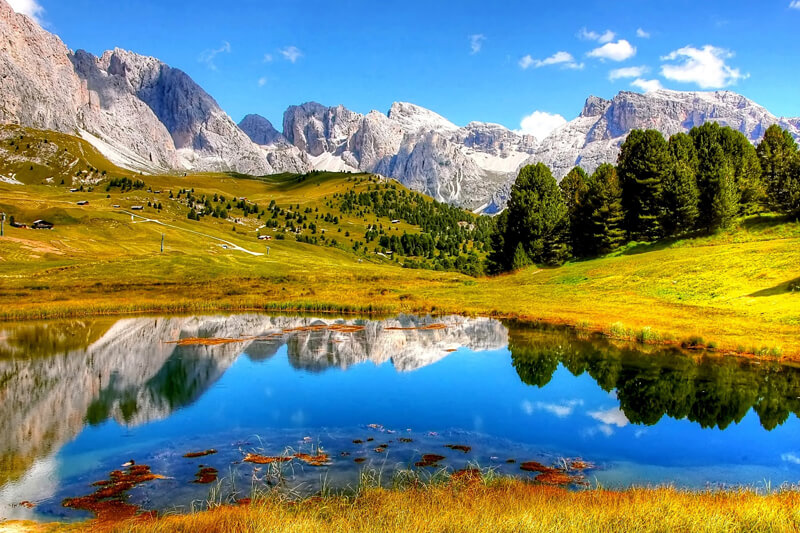
\includegraphics[width=\linewidth]{paisaje.png}\\
\small (a) Original PNG.
\end{minipage}\hfill
\begin{minipage}{0.48\textwidth}
\centering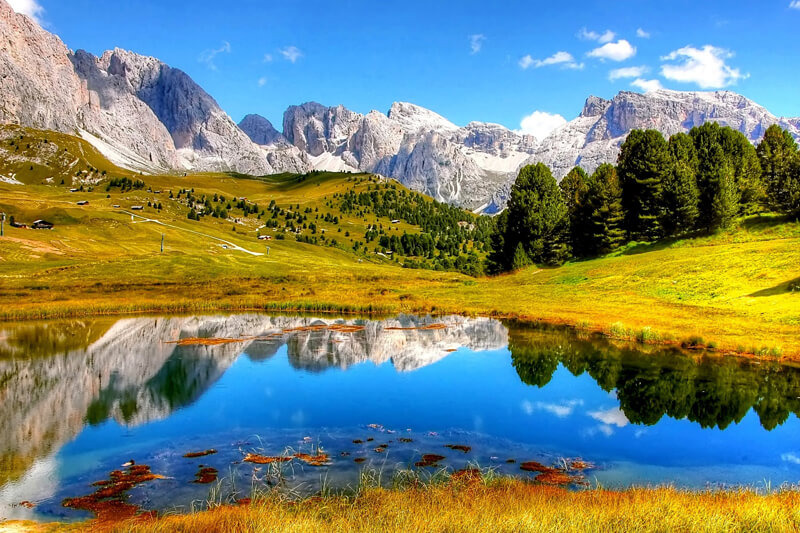
\includegraphics[width=\linewidth]{paisaje.jpg}\\
\small (b) Versi\'on JPG.
\end{minipage}
\caption{Comparaci\'on a igual escala de PNG y JPG. La similitud
visual no implica igualdad de los valores de p\'ixel.}
\label{fig:formatos}
\end{figure}

\subsection{Resultados en escala de grises}
La Figura~\ref{fig:grises} presenta los tres resultados junto con el
original, con el mismo encuadre y tama\~no de visualizaci\'on. NTSC y
OpenCV presentan una apariencia muy similar; el promedio RGB oscurece
especialmente las zonas de vegetaci\'on respecto a las conversiones
ponderadas.
\begin{figure}[htbp]
\centering
\begin{minipage}{0.48\textwidth}
\centering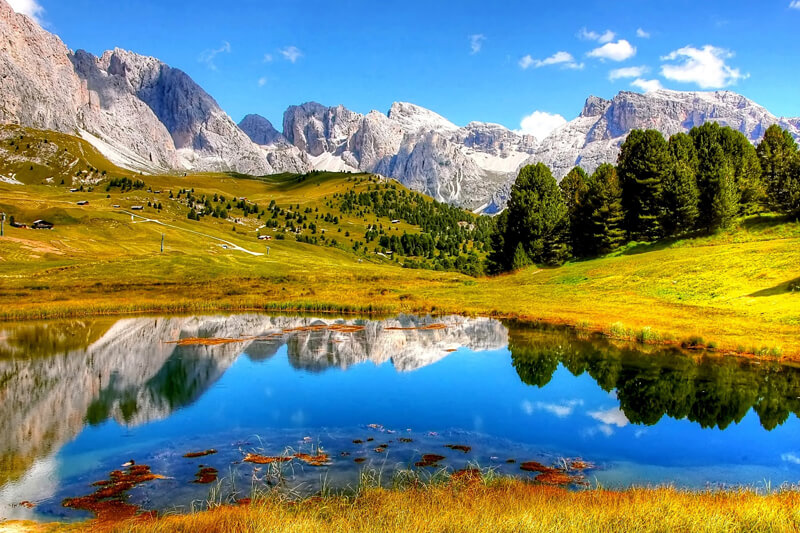
\includegraphics[width=\linewidth]{paisaje.png}\\
\small (a) Original a color.
\end{minipage}\hfill
\begin{minipage}{0.48\textwidth}
\centering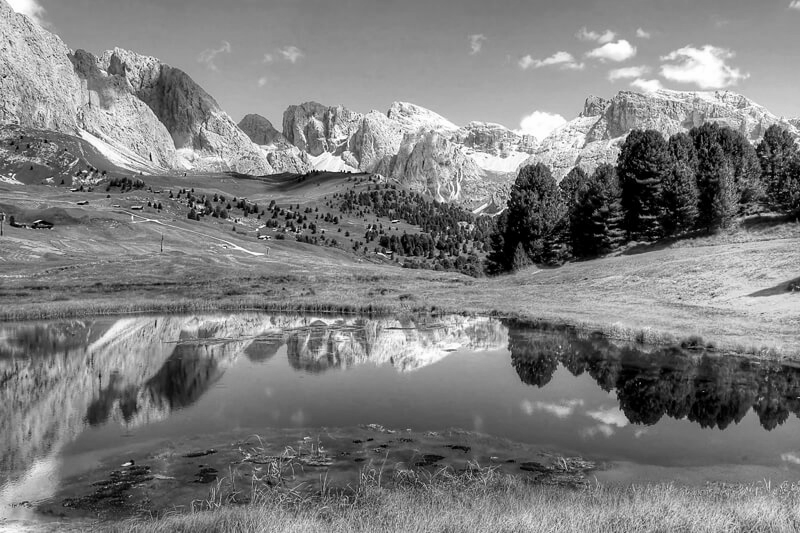
\includegraphics[width=\linewidth]{paisaje_gris_ntsc.png}\\
\small (b) NTSC manual.
\end{minipage}
\par\medskip
\begin{minipage}{0.48\textwidth}
\centering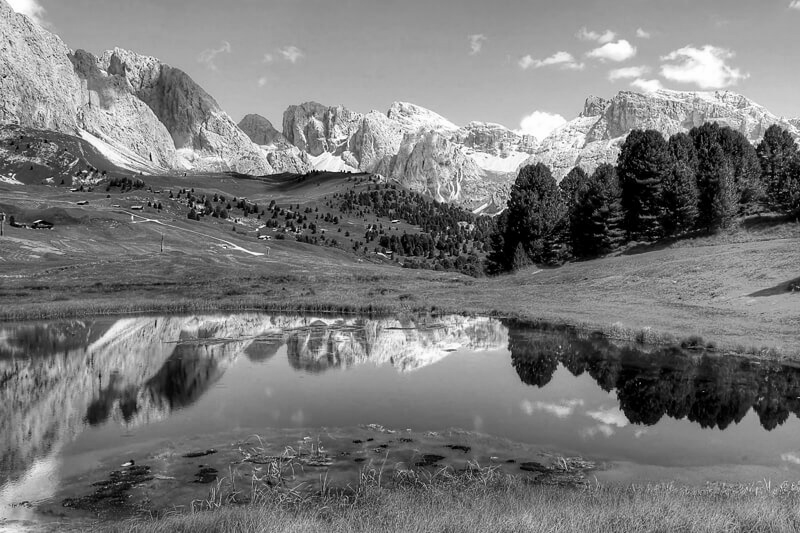
\includegraphics[width=\linewidth]{paisaje_gris_promedio.png}\\
\small (c) Promedio RGB manual.
\end{minipage}\hfill
\begin{minipage}{0.48\textwidth}
\centering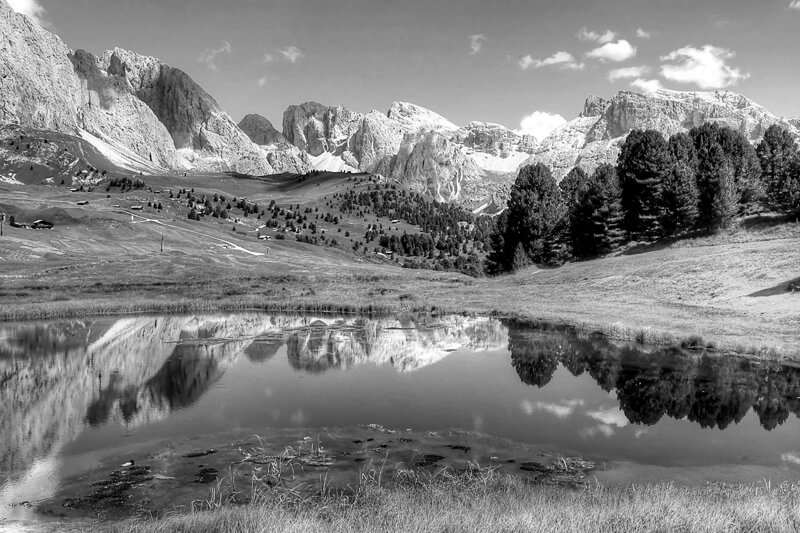
\includegraphics[width=\linewidth]{paisaje_gris.png}\\
\small (d) OpenCV.
\end{minipage}
\caption{Imagen original y conversiones guardadas en la carpeta
\texttt{resultados/}. Las tres salidas conservan la resoluci\'on
espacial de $800\times533$ p\'ixeles.}
\label{fig:grises}
\end{figure}

\subsection{Intensidad promedio (punto 6)}
La Tabla~\ref{tab:brillo} presenta las medias registradas, redondeadas
a seis decimales. Las diferencias se calcularon con los valores completos.
\begin{table}[htbp]
\centering
\caption{Intensidad promedio de las im\'agenes generadas (escala 0--255).}
\label{tab:brillo}
\begin{tabular}{lr}
\toprule
M\'etodo & Intensidad promedio\\
\midrule
NTSC manual & 126.162692\\
Promedio RGB manual & 121.606813\\
OpenCV & 126.699651\\
\bottomrule
\end{tabular}
\end{table}
OpenCV supera la media NTSC en $0.536958$ niveles. NTSC supera al
promedio RGB en $4.555879$ niveles y OpenCV lo supera en $5.092838$.
Adicionalmente, el notebook registra una diferencia absoluta media
NTSC--OpenCV de $0.536958$ y una diferencia absoluta m\'axima de un nivel.
Esta \textit{diferencia absoluta media} compara p\'ixeles correspondientes;
en general no debe confundirse con la diferencia entre las medias.

\section{An\'alisis y conclusiones}
\subsection{Discusi\'on de los resultados}
El archivo JPG es el menor de los cuatro, con $192\,680$ bytes, mientras
que PNG ocupa $876\,700$ bytes. BMP y TIFF se aproximan al volumen de
datos de la matriz sin comprimir, con peque\~nas diferencias atribuibles
a la estructura del archivo y su codificaci\'on. Estas observaciones
corresponden a los archivos evaluados y no establecen una regla universal
sobre el tama\~no de cada formato.

La descompresi\'on explica que archivos de tama\~nos diferentes produzcan
matrices con el mismo consumo de datos en RAM. La compresi\'on en disco
y la representaci\'on de la matriz son aspectos distintos: ninguno de
esos tama\~nos permite, por s\'i solo, determinar la calidad visual.

En la conversi\'on a gris, NTSC y OpenCV asignan al verde un peso cercano
a $0.587$, frente a $0.333$ en el promedio. Por ello, las zonas con
predominio de verde pueden quedar m\'as claras con la ponderaci\'on NTSC.
El resultado global observado es coherente con la presencia de
vegetaci\'on y con las medias medidas. Sin embargo, no se afirma que el
promedio siempre sea m\'as oscuro: en regiones dominadas por azul,
su peso de $0.333$ supera al $0.114$ de NTSC y puede aumentar la intensidad.

La peque\~na discrepancia entre NTSC y OpenCV concuerda con sus
coeficientes cercanos y con las diferencias de cuantizaci\'on.
La diferencia m\'axima registrada de un nivel demuestra que los
resultados no son exactamente iguales, aunque visualmente sean muy
similares. Por su parte, una media resume la imagen completa y no
describe por s\'i sola el contraste ni la distribuci\'on espacial de
las diferencias. Las conclusiones est\'an limitadas al paisaje analizado.

\subsection{Conclusiones}
\begin{enumerate}
\item Los formatos evaluados difieren en tama\~no de archivo, pero la
lectura a color con OpenCV produce matrices de iguales dimensiones,
tipo y cantidad de elementos. Esto no demuestra igualdad de p\'ixeles.
\item JPG fue el archivo m\'as peque\~no y utiliza compresi\'on con
p\'erdida. PNG utiliza compresi\'on sin p\'erdida; BMP y TIFF tuvieron
tama\~nos cercanos al contenido de la matriz sin comprimir en este caso.
\item El orden BGR debe respetarse al aplicar ecuaciones expresadas
en RGB. Las conversiones manuales mediante ciclos permiten hacer
expl\'icita la contribuci\'on de cada canal.
\item NTSC y OpenCV produjeron resultados muy similares, con medias
de $126.162692$ y $126.699651$, respectivamente, y una diferencia
absoluta m\'axima registrada de un nivel.
\item El promedio RGB obtuvo una intensidad media de $121.606813$,
menor que la de las conversiones ponderadas. La diferencia visual en
la vegetaci\'on es consistente con el menor peso asignado al verde.
\item Se guardaron las tres conversiones en PNG. La salida OpenCV
usa un solo canal, mientras que las manuales repiten la intensidad
en tres canales, con mayor ocupaci\'on de datos en memoria.
\end{enumerate}

\begin{thebibliography}{9}
\bibitem{opencv} OpenCV, ``Color conversions'', documentaci\'on de
OpenCV 4.11.0, apartado RGB a escala de grises. Disponible en:
\url{https://docs.opencv.org/4.11.0/de/d25/imgproc_color_conversions.html}.
\end{thebibliography}
\end{document}
